\documentclass[]{article}
\usepackage{lmodern}
\usepackage{amssymb,amsmath}
\usepackage{ifxetex,ifluatex}
\usepackage{fixltx2e} % provides \textsubscript
\ifnum 0\ifxetex 1\fi\ifluatex 1\fi=0 % if pdftex
  \usepackage[T1]{fontenc}
  \usepackage[utf8]{inputenc}
\else % if luatex or xelatex
  \ifxetex
    \usepackage{mathspec}
  \else
    \usepackage{fontspec}
  \fi
  \defaultfontfeatures{Ligatures=TeX,Scale=MatchLowercase}
\fi
% use upquote if available, for straight quotes in verbatim environments
\IfFileExists{upquote.sty}{\usepackage{upquote}}{}
% use microtype if available
\IfFileExists{microtype.sty}{%
\usepackage{microtype}
\UseMicrotypeSet[protrusion]{basicmath} % disable protrusion for tt fonts
}{}
\usepackage[margin=1in]{geometry}
\usepackage{hyperref}
\hypersetup{unicode=true,
            pdftitle={Analyzing Census Data Using R},
            pdfauthor={Corey S. Sparks, Ph.D.},
            pdfborder={0 0 0},
            breaklinks=true}
\urlstyle{same}  % don't use monospace font for urls
\usepackage{color}
\usepackage{fancyvrb}
\newcommand{\VerbBar}{|}
\newcommand{\VERB}{\Verb[commandchars=\\\{\}]}
\DefineVerbatimEnvironment{Highlighting}{Verbatim}{commandchars=\\\{\}}
% Add ',fontsize=\small' for more characters per line
\usepackage{framed}
\definecolor{shadecolor}{RGB}{248,248,248}
\newenvironment{Shaded}{\begin{snugshade}}{\end{snugshade}}
\newcommand{\KeywordTok}[1]{\textcolor[rgb]{0.13,0.29,0.53}{\textbf{#1}}}
\newcommand{\DataTypeTok}[1]{\textcolor[rgb]{0.13,0.29,0.53}{#1}}
\newcommand{\DecValTok}[1]{\textcolor[rgb]{0.00,0.00,0.81}{#1}}
\newcommand{\BaseNTok}[1]{\textcolor[rgb]{0.00,0.00,0.81}{#1}}
\newcommand{\FloatTok}[1]{\textcolor[rgb]{0.00,0.00,0.81}{#1}}
\newcommand{\ConstantTok}[1]{\textcolor[rgb]{0.00,0.00,0.00}{#1}}
\newcommand{\CharTok}[1]{\textcolor[rgb]{0.31,0.60,0.02}{#1}}
\newcommand{\SpecialCharTok}[1]{\textcolor[rgb]{0.00,0.00,0.00}{#1}}
\newcommand{\StringTok}[1]{\textcolor[rgb]{0.31,0.60,0.02}{#1}}
\newcommand{\VerbatimStringTok}[1]{\textcolor[rgb]{0.31,0.60,0.02}{#1}}
\newcommand{\SpecialStringTok}[1]{\textcolor[rgb]{0.31,0.60,0.02}{#1}}
\newcommand{\ImportTok}[1]{#1}
\newcommand{\CommentTok}[1]{\textcolor[rgb]{0.56,0.35,0.01}{\textit{#1}}}
\newcommand{\DocumentationTok}[1]{\textcolor[rgb]{0.56,0.35,0.01}{\textbf{\textit{#1}}}}
\newcommand{\AnnotationTok}[1]{\textcolor[rgb]{0.56,0.35,0.01}{\textbf{\textit{#1}}}}
\newcommand{\CommentVarTok}[1]{\textcolor[rgb]{0.56,0.35,0.01}{\textbf{\textit{#1}}}}
\newcommand{\OtherTok}[1]{\textcolor[rgb]{0.56,0.35,0.01}{#1}}
\newcommand{\FunctionTok}[1]{\textcolor[rgb]{0.00,0.00,0.00}{#1}}
\newcommand{\VariableTok}[1]{\textcolor[rgb]{0.00,0.00,0.00}{#1}}
\newcommand{\ControlFlowTok}[1]{\textcolor[rgb]{0.13,0.29,0.53}{\textbf{#1}}}
\newcommand{\OperatorTok}[1]{\textcolor[rgb]{0.81,0.36,0.00}{\textbf{#1}}}
\newcommand{\BuiltInTok}[1]{#1}
\newcommand{\ExtensionTok}[1]{#1}
\newcommand{\PreprocessorTok}[1]{\textcolor[rgb]{0.56,0.35,0.01}{\textit{#1}}}
\newcommand{\AttributeTok}[1]{\textcolor[rgb]{0.77,0.63,0.00}{#1}}
\newcommand{\RegionMarkerTok}[1]{#1}
\newcommand{\InformationTok}[1]{\textcolor[rgb]{0.56,0.35,0.01}{\textbf{\textit{#1}}}}
\newcommand{\WarningTok}[1]{\textcolor[rgb]{0.56,0.35,0.01}{\textbf{\textit{#1}}}}
\newcommand{\AlertTok}[1]{\textcolor[rgb]{0.94,0.16,0.16}{#1}}
\newcommand{\ErrorTok}[1]{\textcolor[rgb]{0.64,0.00,0.00}{\textbf{#1}}}
\newcommand{\NormalTok}[1]{#1}
\usepackage{graphicx,grffile}
\makeatletter
\def\maxwidth{\ifdim\Gin@nat@width>\linewidth\linewidth\else\Gin@nat@width\fi}
\def\maxheight{\ifdim\Gin@nat@height>\textheight\textheight\else\Gin@nat@height\fi}
\makeatother
% Scale images if necessary, so that they will not overflow the page
% margins by default, and it is still possible to overwrite the defaults
% using explicit options in \includegraphics[width, height, ...]{}
\setkeys{Gin}{width=\maxwidth,height=\maxheight,keepaspectratio}
\IfFileExists{parskip.sty}{%
\usepackage{parskip}
}{% else
\setlength{\parindent}{0pt}
\setlength{\parskip}{6pt plus 2pt minus 1pt}
}
\setlength{\emergencystretch}{3em}  % prevent overfull lines
\providecommand{\tightlist}{%
  \setlength{\itemsep}{0pt}\setlength{\parskip}{0pt}}
\setcounter{secnumdepth}{0}
% Redefines (sub)paragraphs to behave more like sections
\ifx\paragraph\undefined\else
\let\oldparagraph\paragraph
\renewcommand{\paragraph}[1]{\oldparagraph{#1}\mbox{}}
\fi
\ifx\subparagraph\undefined\else
\let\oldsubparagraph\subparagraph
\renewcommand{\subparagraph}[1]{\oldsubparagraph{#1}\mbox{}}
\fi

%%% Use protect on footnotes to avoid problems with footnotes in titles
\let\rmarkdownfootnote\footnote%
\def\footnote{\protect\rmarkdownfootnote}

%%% Change title format to be more compact
\usepackage{titling}

% Create subtitle command for use in maketitle
\newcommand{\subtitle}[1]{
  \posttitle{
    \begin{center}\large#1\end{center}
    }
}

\setlength{\droptitle}{-2em}

  \title{Analyzing Census Data Using R}
    \pretitle{\vspace{\droptitle}\centering\huge}
  \posttitle{\par}
    \author{Corey S. Sparks, Ph.D.}
    \preauthor{\centering\large\emph}
  \postauthor{\par}
      \predate{\centering\large\emph}
  \postdate{\par}
    \date{February 18, 2019}


\begin{document}
\maketitle

{
\setcounter{tocdepth}{2}
\tableofcontents
}
\subsection{Welcome!}\label{welcome}

\subsection{Structure of workshop}\label{structure-of-workshop}

\begin{enumerate}
\def\labelenumi{\arabic{enumi})}
\tightlist
\item
  About me
\item
  Types of census data
\item
  The Census API
\item
  Using \texttt{tidycensus} and \texttt{censusapi} to get data on places
\item
  Using the \texttt{ipumsr} package to get data on people
\end{enumerate}

\subsection{About me}\label{about-me}

I am an associate professor in the
\href{http://copp.utsa.edu/demography/}{UTSA Department of Demography}
and have been at UTSA since 2006.

Research interests include data science, Bayesian methods, education
demography and health disparities. \newpage

\subsection{Types of Census Data}\label{types-of-census-data}

Decennial Census

American Community Survey

County Business Patterns

Population Estimates Program - SAIPE and SAHIE \newpage

\subsubsection{Decennial Census Summary File
1}\label{decennial-census-summary-file-1}

The Census Summary File 1(SF 1) contains the data compiled from the
questions asked of all people and about every housing unit.

Population items include sex, age, race, Hispanic or Latino origin,
household relationship, household type, household size, family type,
family size, and group quarters. Housing items include occupancy status,
vacancy status, and tenure (whether a housing unit is owner-occupied or
renter-occupied).

SF 1 includes population and housing characteristics for the total
population, population totals for an extensive list of race (American
Indian and Alaska Native tribes, Asian, and Native Hawaiian and Other
Pacific Islander) and Hispanic or Latino groups, and population and
housing characteristics for a limited list of race and Hispanic or
Latino groups.

The decennial Census summary file 1 \textbf{\emph{does not}} contain
information on education, socioeconomic conditions or other detailed
characteristics of the population.

Up until 2010, the Census bureau surveyed 1 out of every 6 households to
measure these characteristics, which was referred to as the Census
``long form'', which was tabulated into a product called the Summary
File 3. The year 2000 was the last year this survey was conducted, and
beginning in 2005, the American Community Survey replaced the ``long
form'' as the tool to measure socioeconomic characteristics of the
population. (US Census Bureau, 2010)

\subsubsection{American Community Survey Summary
File}\label{american-community-survey-summary-file}

The American Community Survey (ACS) is part of the U.S. Census Bureau's
Survey Program and is designed to provide current demographic, social,
economic, and housing estimates throughout the decade.

The ACS provides information on more than 40 topics, including
educational attainment, language spoken at home, ability to speak
English, the foreign born, marital status, migration, and many more.
Each year the survey randomly samples around 3.5 million addresses and
produces statistics that cover 1-year and 5-year periods for geographic
areas in the United States and Puerto Rico, ranging from neighborhoods
to congressional districts to the entire nation.

The \textbf{ACS 1-year} estimates are published for areas that have
populations of 65,000 or more.

The \textbf{ACS 5-year} estimates are published for all geographic
areas, including Census tracts, block groups, American Indian areas,
core-based statistical areas, combined statistical areas, Congressional
districts, and state legislative districts.

The American Community Survey Summary File (ACSSF) is a unique data
product that includes all the estimates and margins of error from the
detailed tables and geographies that are published for the ACS. Data
contained in the ACS Summary File cover demographic, social, economic,
and housing subject areas.

These data represent totals of population counts, along with the
measurement errors in those counts for places, not for individuals,
which is the subject of the ACS Public Use Microdata.

\subsubsection{American Community Survey Public Use
Microdata}\label{american-community-survey-public-use-microdata}

The Public Use Microdata Sample \textbf{\emph{(PUMS)}} contains a sample
of actual responses to the American Community Survey (ACS). The PUMS
dataset includes variables for nearly every question on the survey, as
well as many new variables that were derived after the fact from
multiple survey responses (such as poverty status).

Each record in the file represents a \textbf{\emph{single person, or--in
the household-level dataset--a single housing unit}}. In the
person-level file, individuals are organized into households, making
possible the study of people within the contexts of their families and
other household members.

PUMS files for an individual year, such as 2015, contain data on
approximately one percent of the United States population. PUMS files
covering a five-year period, such as 2011-2015, contain data on
approximately five percent of the United States population.

The PUMS files are much more flexible than the aggregate data produced
in the ACS summary files, though the PUMS also tend to be more
complicated to use. Working with PUMS data generally involves
downloading large datasets onto a local computer and analyzing the data
using statistical software such as R, SPSS, Stata, or SAS.

Since all ACS responses are strictly confidential, many variables in the
PUMS files have been modified in order to protect the confidentiality of
survey respondents. For instance, particularly high incomes are
``top-coded,'' uncommon birthplace or ancestry responses are grouped
into broader categories, and the PUMS files provide a very limited set
of geographic variables, including state, metropolitan area and public
use microdata area, or PUMA.

While PUMS files contain cases from nearly every town and county in the
country, towns and counties (and other low-level geography) are not
identified by any variables in the PUMS datasets. The most detailed unit
of geography contained in the PUMS files is the \textbf{\emph{Public Use
Microdata Area (PUMA)}}. PUMAs are special non-overlapping areas that
partition each state into contiguous geographic units containing no
fewer than 100,000 people each. The 2011-2015 5-year ACS PUMS files rely
on PUMA boundaries that were drawn by state governments after the 2000
and 2010 Census.

The PUMS data are most easily accessed from the University of
Minnesota's \textbf{\emph{Integrated Public Use Microdata Series
(IPUMS)}} data archive. This data source processes the data produced by
the Census Bureau into more easily comparable and readable data files
that are available for all years of the decennial Census and the ACS.
(Ruggles et al., 2015)

\newpage

\section{Using the tidycensus
package}\label{using-the-tidycensus-package}

They \href{https://github.com/walkerke/tidycensus}{tidycensus} is part
of the \texttt{tidyverse}, and was written and maintained by
\href{http://personal.tcu.edu/kylewalker/}{Dr.~Kyle Walker} at TCU.

It allows you to dynamically download and map data from the decennial
Census and ACS for any level of
\href{https://www.census.gov/geo/reference/webatlas/}{Census geography},
except blocks!

If you want data on places, this is the easiest way to get it.

\subsubsection{Census table names}\label{census-table-names}

The Census publishes data for places in \textbf{\emph{summary tables}}.
These follow a pattern for their names, you can find a description of
this
\href{https://www.census.gov/programs-surveys/acs/guidance/which-data-tool/table-ids-explained.html}{here}.
The biggest problem with finding data from the Census is knowing the
table name you want.

You can find table names for the ACS
\href{https://www.census.gov/data/developers/data-sets/acs-5year.html}{here}

\subsubsection{What kind of table do you
want?}\label{what-kind-of-table-do-you-want}

There are several types of tables the Census publishes.

The
\href{https://api.census.gov/data/2016/acs/acs5/variables.html}{Detailed
tables} are very detailed summaries of the data for places, in the 2015
data there were more than 64,000 tables published. These can be a little
overwhelming to use, but we'll see an example below

\href{https://api.census.gov/data/2016/acs/acs5/subject.html}{Subject
tables} take some of the detailed tables and compute summaries of them
around certain demographic, social or economic subjects. Basically this
is one way to get more data related to a subject without having to know
all of the individual detail tables you need.

\href{https://api.census.gov/data/2016/acs/acs5/profile.html}{Data
Profile tables} contain broad social, economic, housing, and demographic
information. The data are presented as both counts and percentages.
There are over 2,400 variables in this dataset. These are very useful
summaries and what I personally rely on for most of my data extracts.

\subsubsection{Get a Census developer API
Key}\label{get-a-census-developer-api-key}

Obtain one at \url{http://api.census.gov/data/key_signup.html}

\subsubsection{Save your API key to your working
directory}\label{save-your-api-key-to-your-working-directory}

I recommend you install your API key in your Rprofile, just so you don't
have to keep pasting it into your code. To do this, type
\texttt{tidycensus::census\_api\_key(key\ =\ \ "yourkeyhere",\ install\ =\ T)}
one time to install your key for use in \texttt{tidycensus}.

\subsubsection{Let's do some stuff!}\label{lets-do-some-stuff}

\newpage

\subsubsection{Look at available ACS
variables}\label{look-at-available-acs-variables}

As I mentioned above, finding the right table can be a challenge,
especially for new data users. \texttt{tidycensus} has the
\texttt{load\_variables()} function that will load all of the available
tables for a specific table type.

For example, if we are interested in variables from the ACS
\href{https://www.census.gov/acs/www/data/data-tables-and-tools/data-profiles/2016/}{data
profile} tables, we can load all available variables then use R to
search for what we need.

One of the best ways to search is to use
\href{https://en.wikipedia.org/wiki/Grep}{\texttt{grep()}}, which is a
tool for searching for patterns within text, and is \textbf{\emph{SUPER
USEFUL!}}

\begin{Shaded}
\begin{Highlighting}[]
\KeywordTok{library}\NormalTok{(tidycensus)}
\KeywordTok{library}\NormalTok{(dplyr)}
\KeywordTok{library}\NormalTok{(sf)}
\KeywordTok{library}\NormalTok{(ggplot2)}
\KeywordTok{library}\NormalTok{(censusapi)}
\end{Highlighting}
\end{Shaded}

\begin{Shaded}
\begin{Highlighting}[]
\NormalTok{?load_variables}
\NormalTok{v15_Profile <-}\StringTok{ }\KeywordTok{load_variables}\NormalTok{(}\DataTypeTok{year =} \DecValTok{2015}\NormalTok{ , }\DataTypeTok{dataset =} \StringTok{"acs5/profile"}\NormalTok{,}
                              \DataTypeTok{cache =} \OtherTok{TRUE}\NormalTok{) }\CommentTok{#demographic profile tables}

\CommentTok{#Open the data for examination}
\KeywordTok{View}\NormalTok{(v15_Profile)}

\CommentTok{#Search for variables by keywords in the label}
\NormalTok{v15_Profile[}\KeywordTok{grep}\NormalTok{(}\DataTypeTok{x =}\NormalTok{ v15_Profile}\OperatorTok{$}\NormalTok{label, }\StringTok{"Median household"}\NormalTok{), }\KeywordTok{c}\NormalTok{(}\StringTok{"name"}\NormalTok{, }\StringTok{"label"}\NormalTok{)]}
\end{Highlighting}
\end{Shaded}

\begin{verbatim}
## # A tibble: 2 x 2
##   name       label                                                         
##   <chr>      <chr>                                                         
## 1 DP03_0062  Estimate!!INCOME AND BENEFITS (IN 2015 INFLATION-ADJUSTED DOL~
## 2 DP03_0062P Percent!!INCOME AND BENEFITS (IN 2015 INFLATION-ADJUSTED DOLL~
\end{verbatim}

Also, if you want the names and info for the subject tables, change the
\texttt{dataset\ =} argument to \texttt{acs5/subject}

\begin{Shaded}
\begin{Highlighting}[]
\NormalTok{v15_subject <-}\StringTok{ }\KeywordTok{load_variables}\NormalTok{(}\DataTypeTok{year =} \DecValTok{2015}\NormalTok{ ,}\DataTypeTok{dataset=} \StringTok{"acs5/subject"}\NormalTok{,}
                              \DataTypeTok{cache =} \OtherTok{TRUE}\NormalTok{) }\CommentTok{#demographic subject tables}
\end{Highlighting}
\end{Shaded}

Finally, to view variables in the detailed tables, change the
\texttt{dataset\ =} argument to \texttt{acs5}

\begin{Shaded}
\begin{Highlighting}[]
\NormalTok{v15_detailed <-}\StringTok{ }\KeywordTok{load_variables}\NormalTok{(}\DataTypeTok{year =} \DecValTok{2015}\NormalTok{ , }\DataTypeTok{dataset =} \StringTok{"acs5"}\NormalTok{,}
                               \DataTypeTok{cache =} \OtherTok{TRUE}\NormalTok{) }\CommentTok{#demographic detail tables}
\end{Highlighting}
\end{Shaded}

If you are interested in variables from the decennial census, change the
\texttt{dataset\ =} argument to \texttt{sf1} or \texttt{sf3} depending
on which decennial summary file you want.

\newpage

\subsection{Extract from ACS summary file data profile variables from
2015 for Bexar County, TX Census
Tracts}\label{extract-from-acs-summary-file-data-profile-variables-from-2015-for-bexar-county-tx-census-tracts}

Here is a real example

The data profile tables are very useful because they contain lots of
pre-calculated variables.

Here is a query where we extract the median household income in census
tracts from the 2015 ACS for Bexar County, Texas. We can also get the
spatial data by requesting \texttt{geometry=TRUE}. Using
\texttt{output="wide"} will put each variable in a column of the data
set, with each row being a census tract.

\begin{Shaded}
\begin{Highlighting}[]
\NormalTok{sa_acs<-}\KeywordTok{get_acs}\NormalTok{(}\DataTypeTok{geography =} \StringTok{"tract"}\NormalTok{, }\DataTypeTok{state=}\StringTok{"TX"}\NormalTok{, }\DataTypeTok{county =} \StringTok{"Bexar"}\NormalTok{,}
                \DataTypeTok{year =} \DecValTok{2015}\NormalTok{,}
                \DataTypeTok{variables=}\KeywordTok{c}\NormalTok{( }\StringTok{"DP03_0062E"}\NormalTok{) ,}
                \DataTypeTok{geometry =}\NormalTok{ T, }\DataTypeTok{output =} \StringTok{"wide"}\NormalTok{)}
\end{Highlighting}
\end{Shaded}

\begin{verbatim}
## Getting data from the 2011-2015 5-year ACS
\end{verbatim}

\begin{verbatim}
## Downloading feature geometry from the Census website.  To cache shapefiles for use in future sessions, set `options(tigris_use_cache = TRUE)`.
\end{verbatim}

\begin{verbatim}
## Using the ACS Data Profile
\end{verbatim}

\begin{Shaded}
\begin{Highlighting}[]
\CommentTok{#create a county FIPS code - 5 digit}
\NormalTok{sa_acs}\OperatorTok{$}\NormalTok{county<-}\KeywordTok{substr}\NormalTok{(sa_acs}\OperatorTok{$}\NormalTok{GEOID, }\DecValTok{1}\NormalTok{, }\DecValTok{5}\NormalTok{)}

\CommentTok{#rename variables and filter missing cases}
\NormalTok{sa_acs2<-sa_acs}\OperatorTok
\StringTok{  }\KeywordTok{mutate}\NormalTok{( }\DataTypeTok{medhhinc=}\NormalTok{DP03_0062E) }\OperatorTok
\StringTok{  }\KeywordTok{na.omit}\NormalTok{()}

\CommentTok{#take a peek at the first few lines of data}
\KeywordTok{head}\NormalTok{(sa_acs2)}
\end{Highlighting}
\end{Shaded}

We can immediately map these data as well, because \texttt{tidycensus}
can get you the geography corresponding to your data.

Here, I use the \texttt{dplyr} pipe ``\texttt{\%\textgreater{}\%}'' to
feed the data into \texttt{ggplot} and map the median household income
for each census tract in Bexar County in 2015, using a quantile break
system.

\begin{Shaded}
\begin{Highlighting}[]
\NormalTok{sa_acs2 }\OperatorTok
\StringTok{  }\KeywordTok{mutate}\NormalTok{(}\DataTypeTok{med_income=}\KeywordTok{cut}\NormalTok{(medhhinc,}
                        \DataTypeTok{breaks =} \KeywordTok{quantile}\NormalTok{(medhhinc, }\DataTypeTok{na.rm=}\NormalTok{T, }\DataTypeTok{p=}\KeywordTok{seq}\NormalTok{(}\DecValTok{0}\NormalTok{,}\DecValTok{1}\NormalTok{,}\DataTypeTok{length.out =} \DecValTok{9}\NormalTok{)),}\DataTypeTok{include.lowest =}\NormalTok{ T))}\OperatorTok
\StringTok{  }\KeywordTok{ggplot}\NormalTok{( }\KeywordTok{aes}\NormalTok{(}\DataTypeTok{fill =}\NormalTok{ med_income, }\DataTypeTok{color =}\NormalTok{ med_income)) }\OperatorTok{+}\StringTok{ }
\StringTok{  }\KeywordTok{geom_sf}\NormalTok{() }\OperatorTok{+}\StringTok{ }
\StringTok{  }\KeywordTok{ggtitle}\NormalTok{(}\StringTok{"Median Household Income"}\NormalTok{, }
          \DataTypeTok{subtitle =} \StringTok{"Bexar County Texas, 2015 - Quantile Breaks"}\NormalTok{)}\OperatorTok{+}
\StringTok{  }\KeywordTok{scale_fill_brewer}\NormalTok{(}\DataTypeTok{palette =} \StringTok{"Blues"}\NormalTok{) }\OperatorTok{+}\StringTok{ }
\StringTok{  }\KeywordTok{scale_color_brewer}\NormalTok{(}\DataTypeTok{palette =} \StringTok{"Blues"}\NormalTok{)}
\end{Highlighting}
\end{Shaded}

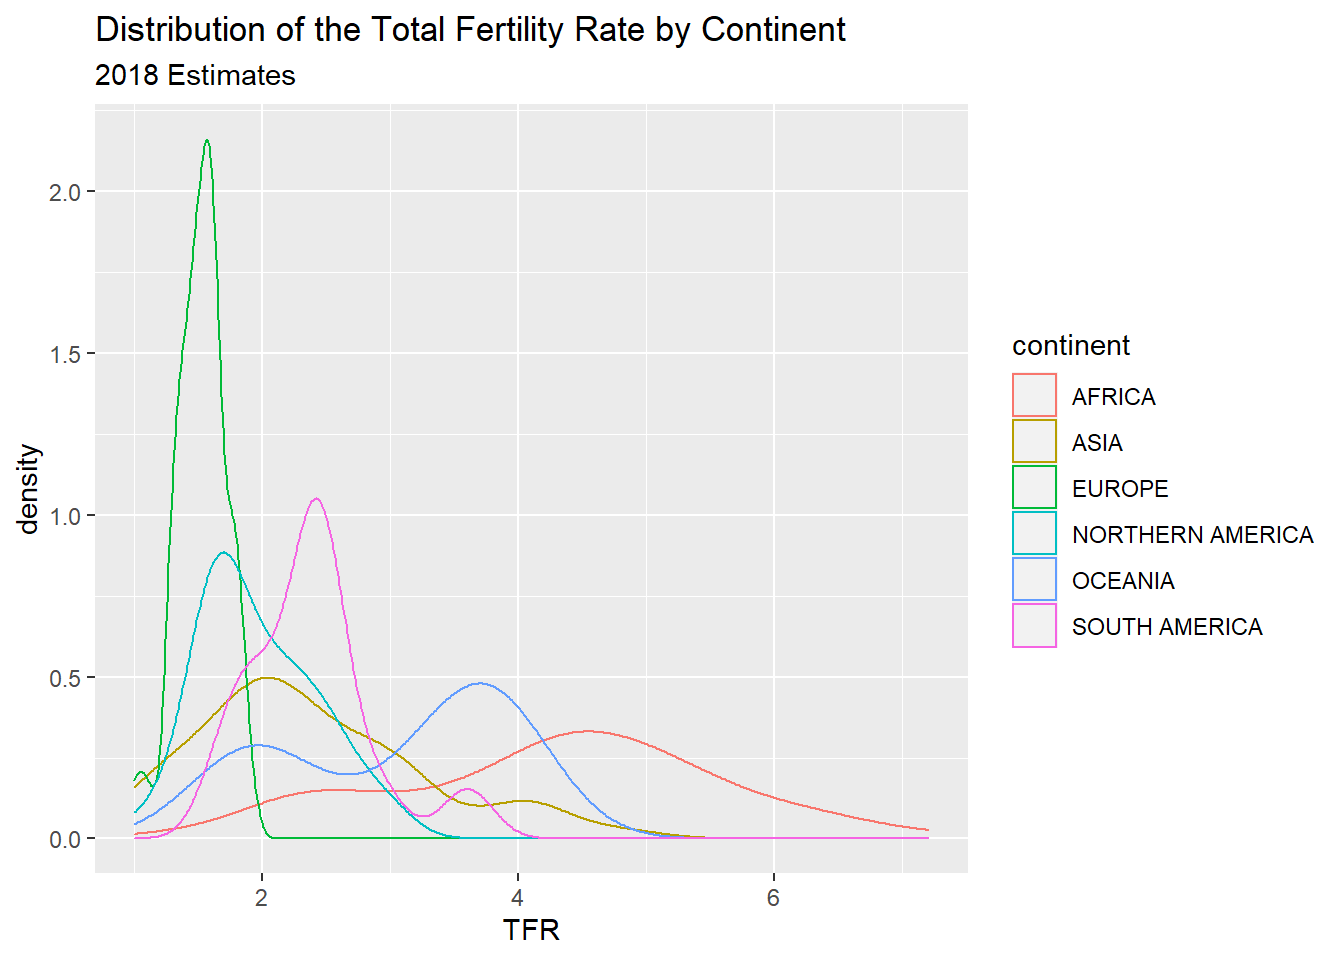
\includegraphics{UTSA_census_workshop_feb19_pdf_files/figure-latex/unnamed-chunk-7-1.pdf}

\newpage

\subsubsection{ACS margins of error}\label{acs-margins-of-error}

The ACS is a survey and in areas where the sample size is small, the
errors in estimates can be quite large. As a way to let users know how
uncertain the estimates are for any given area, the Census publishes
\textbf{\emph{Margins of Error}} for each estimate published. In states,
counties and cities, these margins of error are usually small since the
overall sample size in those larger areas is large enough to provide
more certainty about the population estimates.

In areas that are smaller, tracts and especially block groups, the
margins of error can be be very large relative to the estimates. One way
to visualize this is to map the \textbf{\emph{coefficient of variation}}
in the estimates, which is: \(CV= \frac{\sigma}{\theta}\), where
\(\theta\) is the estimate of interest.

\paragraph{mapping of errors in
variables}\label{mapping-of-errors-in-variables}

Here I generate a quantile break for the coefficient of variation in
census tract income estimates

\begin{Shaded}
\begin{Highlighting}[]
\NormalTok{sa_acs2 }\OperatorTok
\StringTok{  }\KeywordTok{mutate}\NormalTok{(}\DataTypeTok{cv =}\NormalTok{(DP03_0062M}\OperatorTok{/}\FloatTok{1.645}\NormalTok{)}\OperatorTok{/}\NormalTok{DP03_0062E)}\OperatorTok
\StringTok{  }\KeywordTok{mutate}\NormalTok{(}\DataTypeTok{cv_map=}\KeywordTok{cut}\NormalTok{(cv,}
                    \DataTypeTok{breaks =} \KeywordTok{quantile}\NormalTok{(cv, }\DataTypeTok{na.rm=}\NormalTok{T, }\DataTypeTok{p=}\KeywordTok{seq}\NormalTok{(}\DecValTok{0}\NormalTok{,}\DecValTok{1}\NormalTok{,}\DataTypeTok{length.out =} \DecValTok{9}\NormalTok{)),}\DataTypeTok{include.lowest =}\NormalTok{ T))}\OperatorTok
\StringTok{  }\KeywordTok{ggplot}\NormalTok{( }\KeywordTok{aes}\NormalTok{(}\DataTypeTok{fill =}\NormalTok{cv_map, }\DataTypeTok{color =}\NormalTok{ cv_map)) }\OperatorTok{+}\StringTok{ }
\StringTok{  }\KeywordTok{geom_sf}\NormalTok{() }\OperatorTok{+}\StringTok{ }
\StringTok{  }\KeywordTok{ggtitle}\NormalTok{(}\StringTok{"Coefficient of Variation in Median Household Income"}\NormalTok{, }
          \DataTypeTok{subtitle =} \StringTok{"Bexar County Texas, 2015 - Quantile Breaks"}\NormalTok{)}\OperatorTok{+}
\StringTok{  }\KeywordTok{scale_fill_viridis_d}\NormalTok{(}\DataTypeTok{option=}\StringTok{"B"}\NormalTok{)}\OperatorTok{+}\StringTok{ }
\StringTok{  }\KeywordTok{scale_color_viridis_d}\NormalTok{(}\DataTypeTok{option=}\StringTok{"B"}\NormalTok{)}
\end{Highlighting}
\end{Shaded}

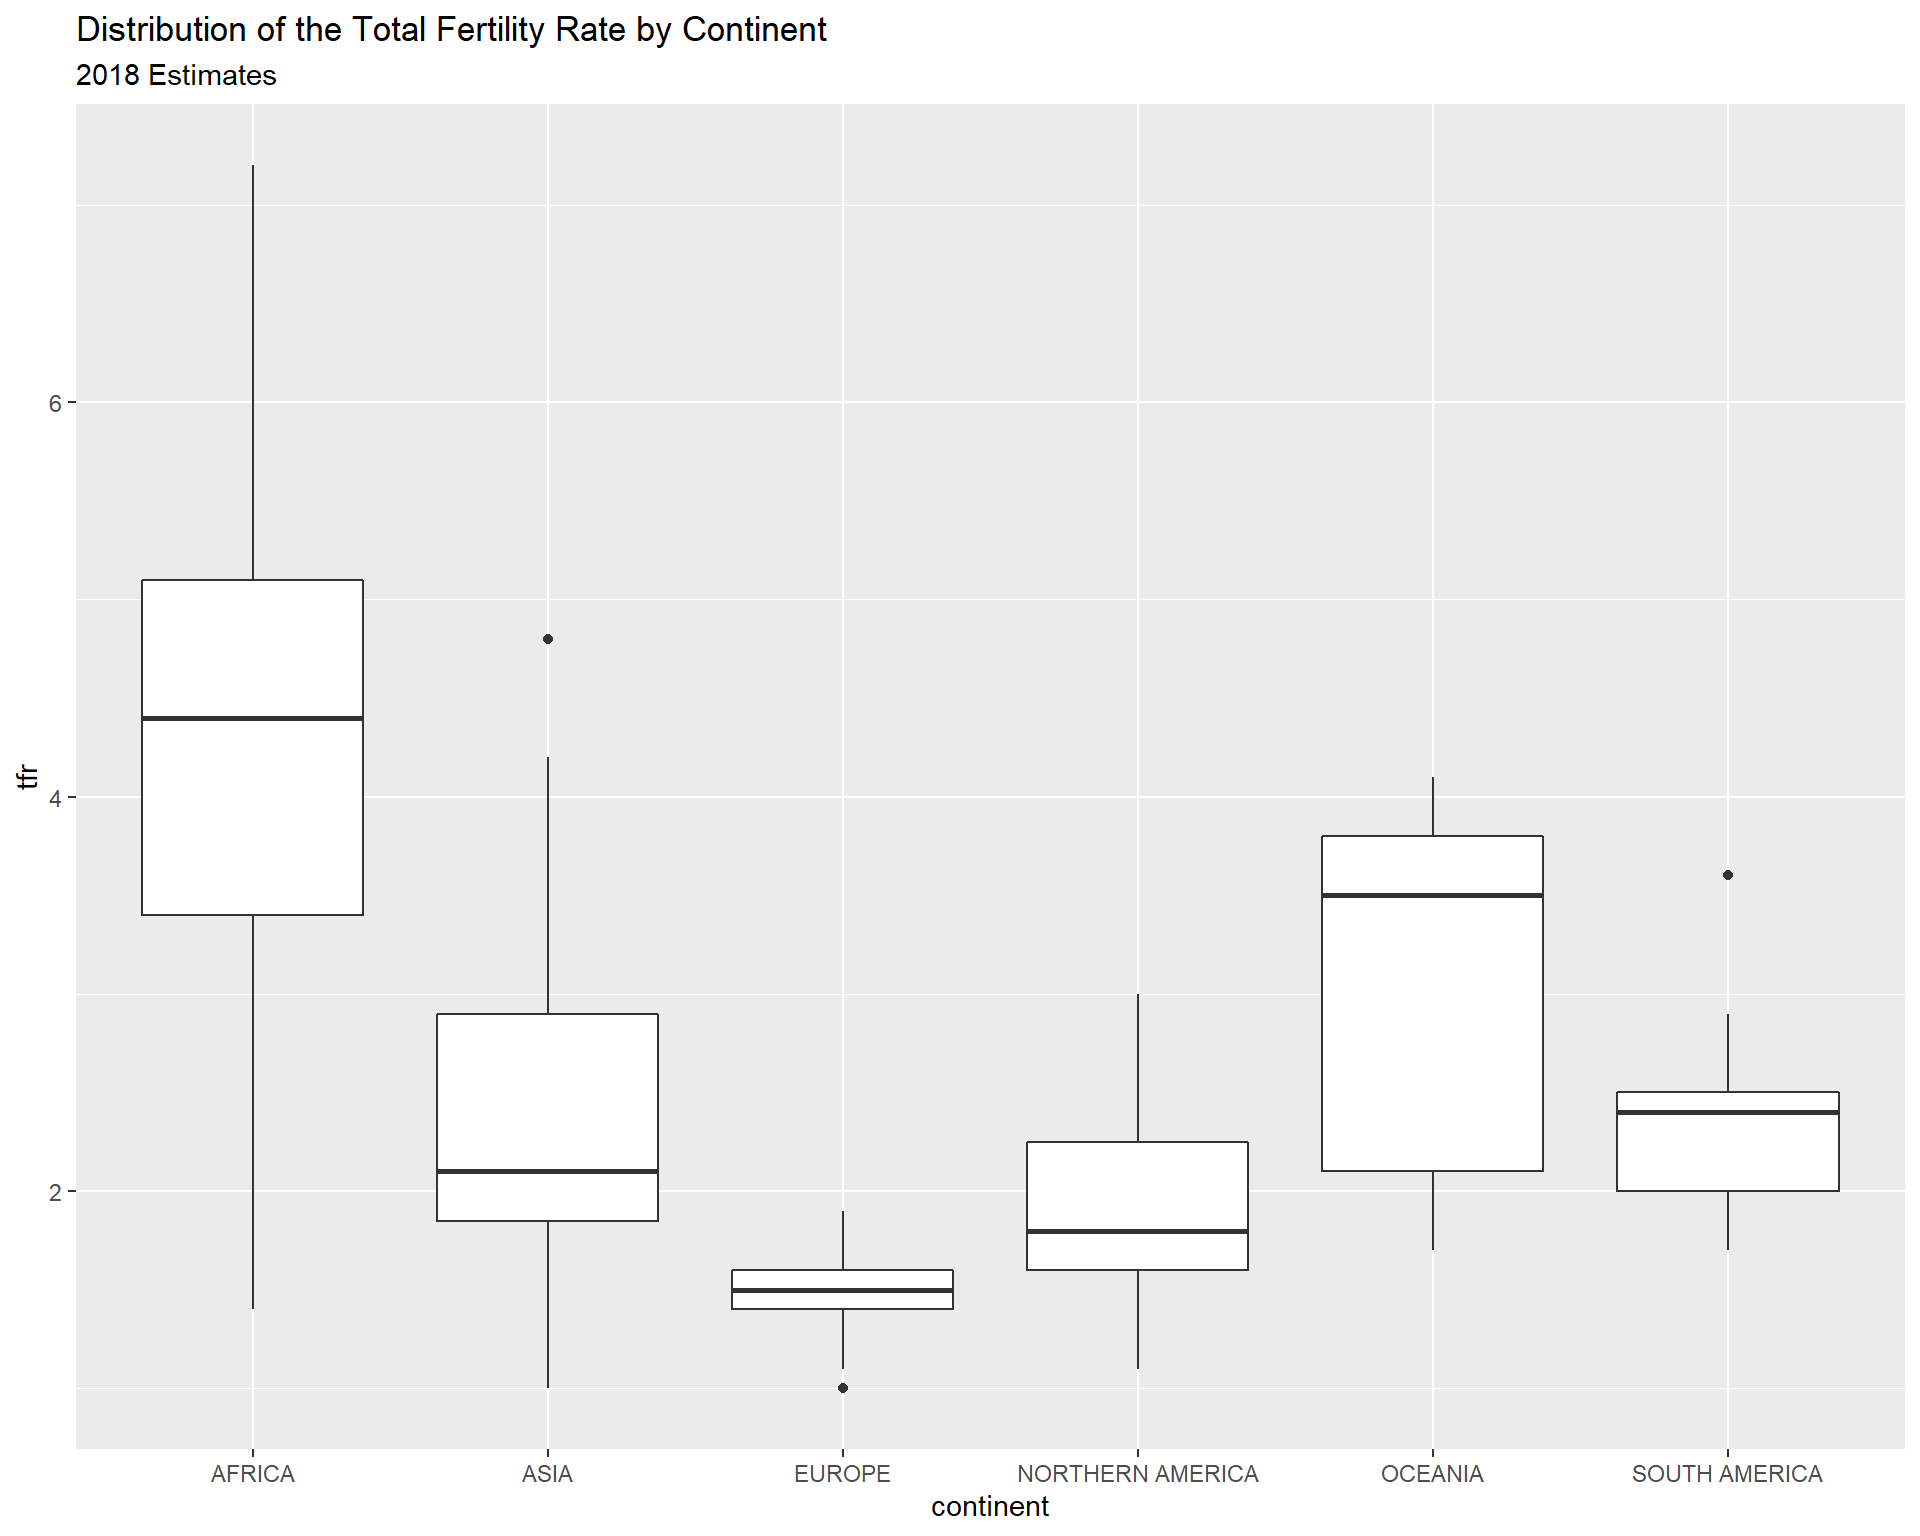
\includegraphics{UTSA_census_workshop_feb19_pdf_files/figure-latex/unnamed-chunk-8-1.pdf}

\newpage

\subsubsection{Metro area incomes}\label{metro-area-incomes}

Here is another example where we get data for metro/micropolitan areas
in the US. I use a detailed table request this time.

\begin{Shaded}
\begin{Highlighting}[]
\NormalTok{v15_acs<-}\StringTok{ }\KeywordTok{load_variables}\NormalTok{(}\DataTypeTok{year =} \DecValTok{2015}\NormalTok{ , }\DataTypeTok{dataset =} \StringTok{"acs5"}\NormalTok{,}
                         \DataTypeTok{cache =} \OtherTok{TRUE}\NormalTok{) }\CommentTok{#regular ACS profile tables}

\KeywordTok{View}\NormalTok{(v15_acs)}

\CommentTok{#Search for variables by keywords in the label }
\NormalTok{v15_acs[}\KeywordTok{grep}\NormalTok{(}\DataTypeTok{x =}\NormalTok{ v15_Profile}\OperatorTok{$}\NormalTok{label, }\StringTok{"Median household"}\NormalTok{), }\KeywordTok{c}\NormalTok{(}\StringTok{"name"}\NormalTok{, }\StringTok{"label"}\NormalTok{)]}

\NormalTok{metro<-}\KeywordTok{get_acs}\NormalTok{(}\DataTypeTok{geography =} \StringTok{"metropolitan statistical area/micropolitan statistical area"}\NormalTok{,}
               \DataTypeTok{year =} \DecValTok{2015}\NormalTok{,}
                \DataTypeTok{variables=}\KeywordTok{c}\NormalTok{( }\StringTok{"B19013_001E"}\NormalTok{) ,}
                \DataTypeTok{geometry =}\NormalTok{ F, }\DataTypeTok{output =} \StringTok{"wide"}\NormalTok{)}
\end{Highlighting}
\end{Shaded}

\begin{verbatim}
## Getting data from the 2011-2015 5-year ACS
\end{verbatim}

For this geography, \texttt{tidycensus} won't download the geometrys
automatically (maybe in a later release), so we use Kyle Walker's other
library \texttt{tigris} for downloading Census geographic data.

\begin{Shaded}
\begin{Highlighting}[]
\KeywordTok{library}\NormalTok{(tigris)}
\end{Highlighting}
\end{Shaded}

\begin{verbatim}
## To enable 
## caching of data, set `options(tigris_use_cache = TRUE)` in your R script or .Rprofile.
\end{verbatim}

\begin{verbatim}
## 
## Attaching package: 'tigris'
\end{verbatim}

\begin{verbatim}
## The following object is masked from 'package:graphics':
## 
##     plot
\end{verbatim}

\begin{Shaded}
\begin{Highlighting}[]
\KeywordTok{options}\NormalTok{(}\DataTypeTok{tigris_class =} \StringTok{"sf"}\NormalTok{) }\CommentTok{#for use with ggplot2}

\NormalTok{met_geo<-}\KeywordTok{core_based_statistical_areas}\NormalTok{(}\DataTypeTok{cb=}\NormalTok{T, }\DataTypeTok{year =} \DecValTok{2015}\NormalTok{)}

\CommentTok{#Filter out territories}
\NormalTok{sts<-}\KeywordTok{states}\NormalTok{(}\DataTypeTok{cb =}\NormalTok{ T, }\DataTypeTok{year =} \DecValTok{2015}\NormalTok{)}\OperatorTok
\StringTok{  }\KeywordTok{filter}\NormalTok{(}\OperatorTok{!}\NormalTok{STATEFP}\OperatorTok\KeywordTok{c}\NormalTok{( }\StringTok{"60"}\NormalTok{, }\StringTok{"66"}\NormalTok{, }\StringTok{"69"}\NormalTok{, }\StringTok{"72"}\NormalTok{, }\StringTok{"78"}\NormalTok{))}

\CommentTok{#merge geographic data to table data}
\NormalTok{met_join<-}\KeywordTok{geo_join}\NormalTok{(met_geo, metro, }\DataTypeTok{by=}\StringTok{"GEOID"}\NormalTok{)}
\end{Highlighting}
\end{Shaded}

\begin{verbatim}
## Warning: st_crs<- : replacing crs does not reproject data; use st_transform
## for that
\end{verbatim}

\begin{Shaded}
\begin{Highlighting}[]
\CommentTok{#rename variables and filter missing cases}
\NormalTok{met_join<-met_join}\OperatorTok
\StringTok{  }\KeywordTok{mutate}\NormalTok{( }\DataTypeTok{medhhinc=}\NormalTok{B19013_001E) }\OperatorTok
\StringTok{  }\KeywordTok{mutate}\NormalTok{(}\DataTypeTok{med_income=}\KeywordTok{cut}\NormalTok{(medhhinc,}
                        \DataTypeTok{breaks =} \KeywordTok{quantile}\NormalTok{(medhhinc, }\DataTypeTok{na.rm=}\NormalTok{T, }\DataTypeTok{p=}\KeywordTok{seq}\NormalTok{(}\DecValTok{0}\NormalTok{,}\DecValTok{1}\NormalTok{,}\DataTypeTok{length.out =} \DecValTok{9}\NormalTok{)),}\DataTypeTok{include.lowest =}\NormalTok{ T))}

\NormalTok{##Create our map}

\NormalTok{map1<-met_join}\OperatorTok
\StringTok{  }\KeywordTok{st_transform}\NormalTok{(}\DataTypeTok{crs =} \DecValTok{102740}\NormalTok{)}\OperatorTok
\StringTok{  }\KeywordTok{ggplot}\NormalTok{( }\KeywordTok{aes}\NormalTok{(}\DataTypeTok{fill =}\NormalTok{ med_income, }\DataTypeTok{color =}\NormalTok{ med_income)) }\OperatorTok{+}\StringTok{ }
\StringTok{  }\KeywordTok{geom_sf}\NormalTok{() }\OperatorTok{+}\StringTok{ }
\StringTok{  }\KeywordTok{ggtitle}\NormalTok{(}\StringTok{"Median Household Income"}\NormalTok{, }
          \DataTypeTok{subtitle =} \StringTok{"MSAs, 2015 - Quantile Breaks"}\NormalTok{)}\OperatorTok{+}
\StringTok{  }\KeywordTok{scale_fill_brewer}\NormalTok{(}\DataTypeTok{palette =} \StringTok{"Blues"}\NormalTok{) }\OperatorTok{+}\StringTok{ }
\StringTok{  }\KeywordTok{scale_color_brewer}\NormalTok{(}\DataTypeTok{palette =} \StringTok{"Blues"}\NormalTok{)}\OperatorTok{+}
\StringTok{  }\KeywordTok{geom_sf}\NormalTok{(}\DataTypeTok{data=}\NormalTok{sts, }\DataTypeTok{fill=}\OtherTok{NA}\NormalTok{, }\DataTypeTok{color=}\StringTok{"black"}\NormalTok{)}
    
\NormalTok{map1}
\end{Highlighting}
\end{Shaded}

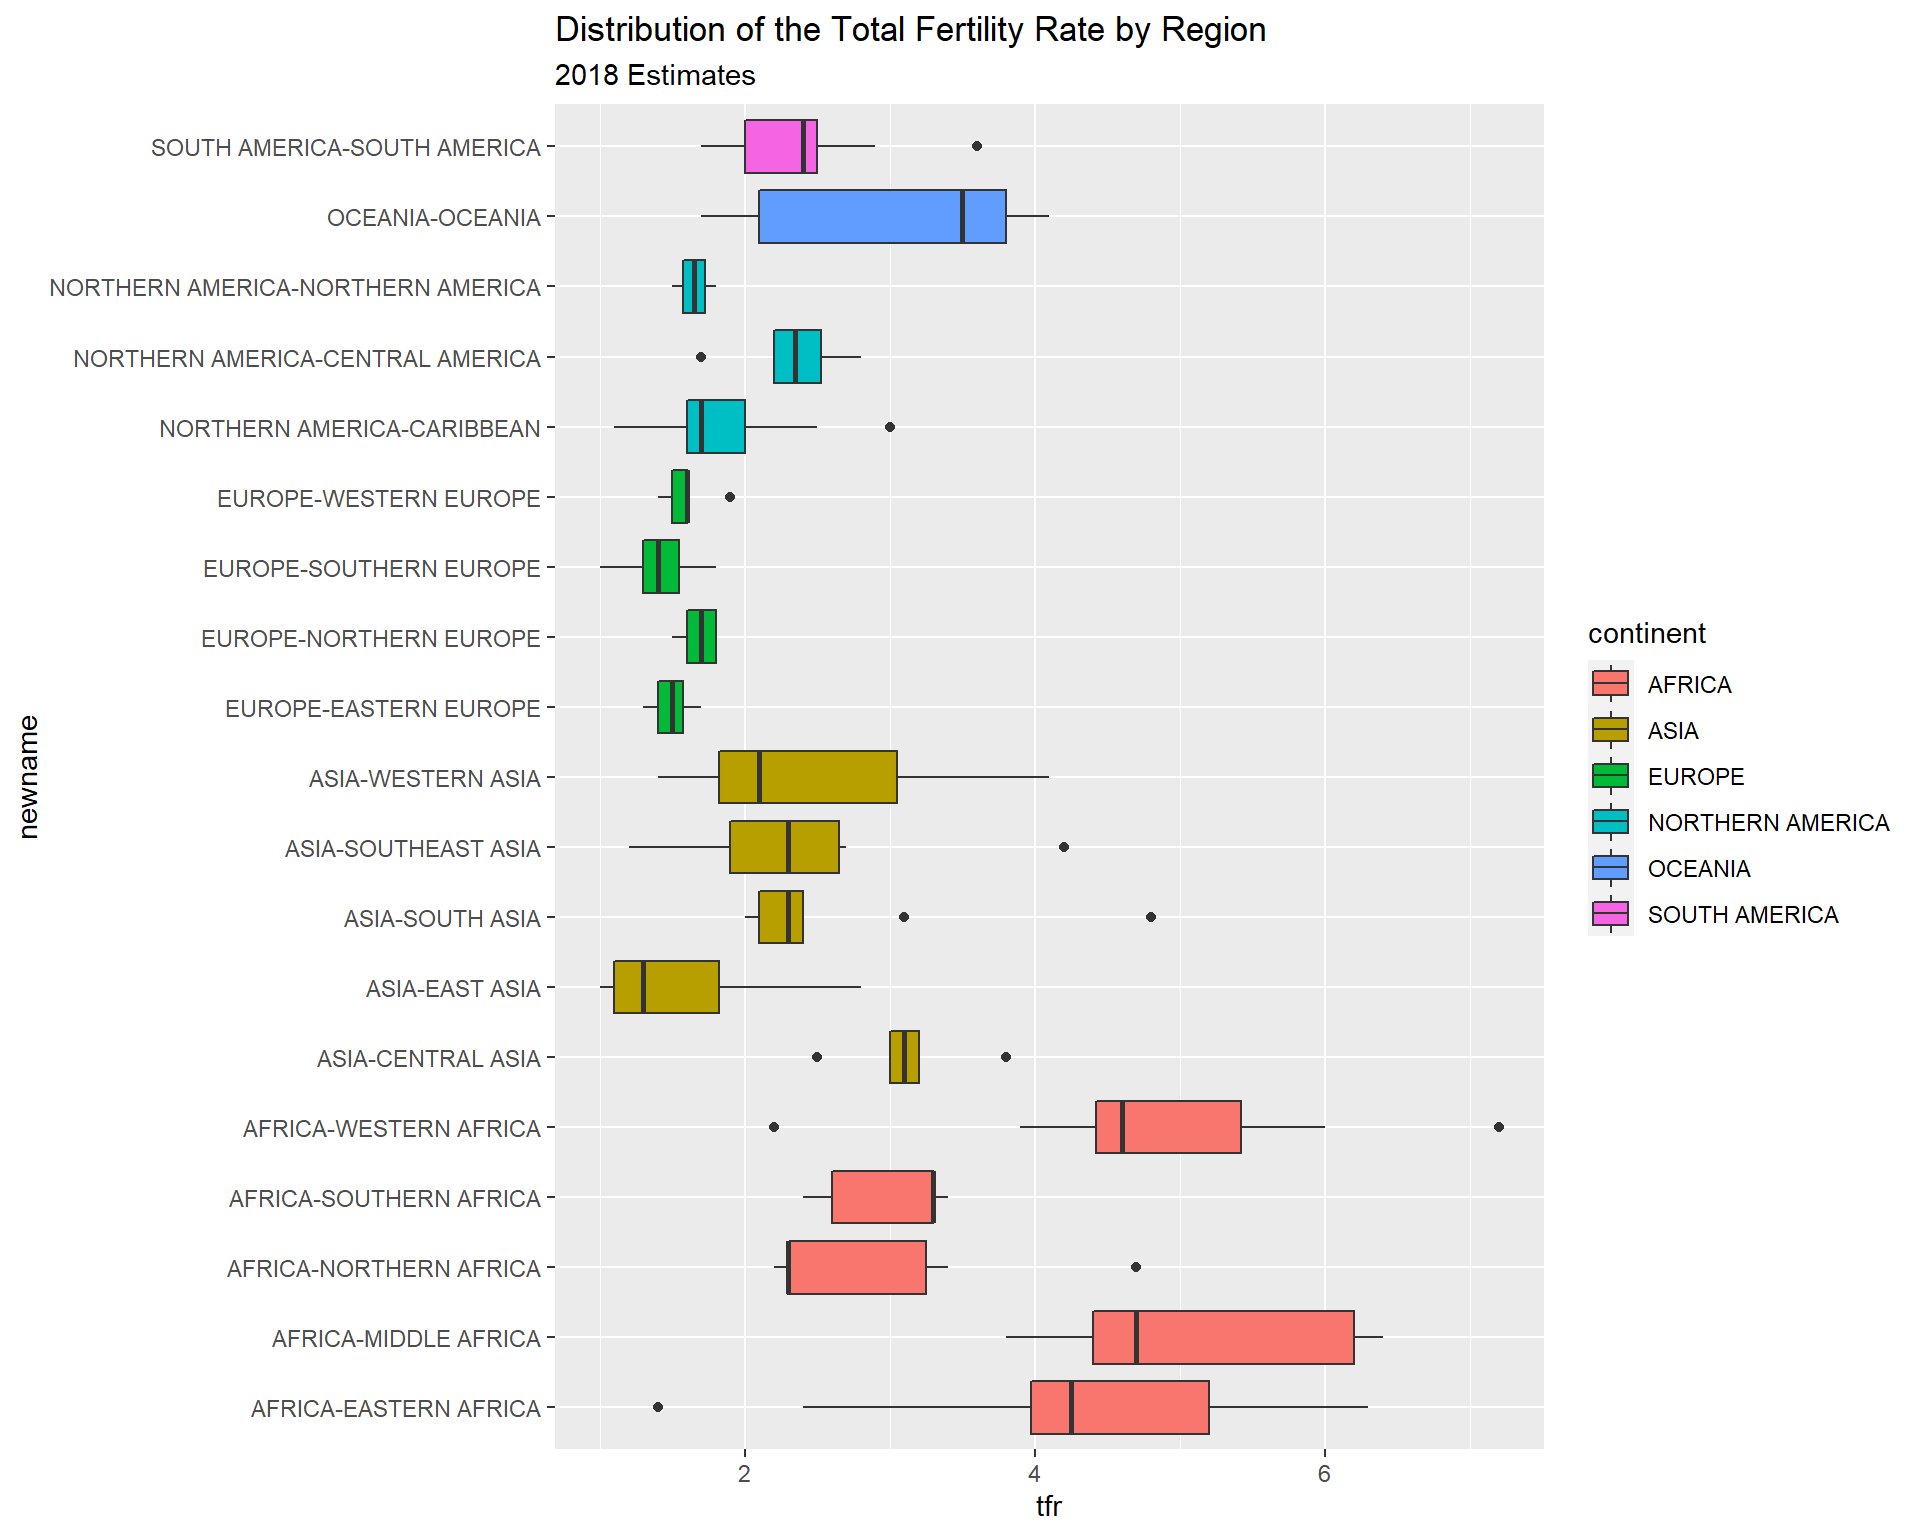
\includegraphics{UTSA_census_workshop_feb19_pdf_files/figure-latex/unnamed-chunk-10-1.pdf}

If you would like to zoom in, we can use the \texttt{mapview} library.
This is very useful for teaching and for presentations.

\begin{Shaded}
\begin{Highlighting}[]
\KeywordTok{library}\NormalTok{(mapview)}

\NormalTok{pal <-}\StringTok{ }\KeywordTok{colorRampPalette}\NormalTok{(viridisLite}\OperatorTok{::}\KeywordTok{viridis}\NormalTok{(}\DataTypeTok{n=}\DecValTok{6}\NormalTok{)) }\CommentTok{#set colors}

\KeywordTok{mapview}\NormalTok{(met_join, }\DataTypeTok{zcol=}\StringTok{"med_income"}\NormalTok{, }\DataTypeTok{col.regions=}\NormalTok{pal, }\DataTypeTok{legend=}\NormalTok{T,}\DataTypeTok{map.types=}\StringTok{"OpenStreetMap"}\NormalTok{, }\DataTypeTok{layer.name=}\StringTok{"Median Income"}\NormalTok{)}
\end{Highlighting}
\end{Shaded}

\begin{verbatim}
## PhantomJS not found. You can install it with webshot::install_phantomjs(). If it is installed, please make sure the phantomjs executable can be found via the PATH variable.
\end{verbatim}

\hypertarget{htmlwidget-e8faa941690678c3ca3f}{}

\newpage

\section{Using the censusapi package}\label{using-the-censusapi-package}

The Census has lots of APIs that are available. \texttt{tidycensus} is
great for accessing the ACS and decennial census, but if you want data
from another API, the more general \texttt{censusapi} package gives you
access to all of the Census APIs

First, since this is a different package, you'll need to add your API
key to your \texttt{.Renviron} data. You can do this by following the
example below:

\begin{Shaded}
\begin{Highlighting}[]
\KeywordTok{Sys.setenv}\NormalTok{(}\DataTypeTok{CENSUS_KEY=}\StringTok{"yourkeyhere"}\NormalTok{)}
\CommentTok{# Reload .Renviron}
\KeywordTok{readRenviron}\NormalTok{(}\StringTok{"~/.Renviron"}\NormalTok{)}
\CommentTok{# Check to see that the expected key is output in your R console}
\KeywordTok{Sys.getenv}\NormalTok{(}\StringTok{"CENSUS_KEY"}\NormalTok{)}
\end{Highlighting}
\end{Shaded}

Now we load all of the available APIs into an R object so we can look
what's available.

\begin{Shaded}
\begin{Highlighting}[]
\NormalTok{apis <-}\StringTok{ }\KeywordTok{listCensusApis}\NormalTok{()}
\KeywordTok{View}\NormalTok{(apis)}
\end{Highlighting}
\end{Shaded}

So, we can see there are a lot. For a concrete example, let's examine
the effect of the
\href{https://en.wikipedia.org/wiki/Patient_Protection_and_Affordable_Care_Act}{Patient
Protection and Affordable Care Act} on uninsurance rates in US states.

For this, we will use the
\href{https://www.census.gov/programs-surveys/sahie.html}{Small Area
Health Insurance Estimates} program. This program combines data from the
ACS and data from individual states on other health insurance programs
to produce model-based estimates of the overall rates of insurance and
uninsurance for states and counties.

Census maintains a nice
\href{https://www.census.gov/data-tools/demo/sahie/\#/}{website} for
browsing the data and downloading images of data visualizations, but
anything custom can be a process. In R this is no problem.

Below, we first look up the variables available in the SAHIE data, then
we do an extract and create a dataset for Texas and California for
unsinsurance rates by race/ethnicity. Next, we create a line plot of the
uninsurance time series for each state and demographic group.

\begin{Shaded}
\begin{Highlighting}[]
\CommentTok{#timeseries/poverty/saipe}
\NormalTok{sahevars<-}\KeywordTok{listCensusMetadata}\NormalTok{(}\DataTypeTok{name =} \StringTok{"timeseries/healthins/sahie"}\NormalTok{, }\DataTypeTok{type =} \StringTok{"v"}\NormalTok{)}
\KeywordTok{head}\NormalTok{(sahevars)}
\end{Highlighting}
\end{Shaded}

\begin{verbatim}
##       name                                                           label
## 1 AGE_DESC                                        Age Category Description
## 2 NUI_LB90       Number Uninsured, Lower Bound for 90% Confidence Interval
## 3    STATE                                                 State FIPS Code
## 4  NIC_MOE                                 Number Insured, Margin of Error
## 5  NIPR_PT Number in Demographic Group for Selected Income Range, Estimate
## 6  RACECAT                                                   Race Category
##               concept predicateType group limit          required
## 1      Demographic ID           int   N/A     0              <NA>
## 2 Uncertainty Measure           int   N/A     0              <NA>
## 3       Geographic ID           int   N/A     0              <NA>
## 4 Uncertainty Measure           int   N/A     0              <NA>
## 5            Estimate           int   N/A     0              <NA>
## 6      Demographic ID           int   N/A     0 default displayed
\end{verbatim}

\begin{Shaded}
\begin{Highlighting}[]
\CommentTok{#SAEPOVRTALL_PT}
\end{Highlighting}
\end{Shaded}

\subsubsection{Get the data for states}\label{get-the-data-for-states}

\begin{Shaded}
\begin{Highlighting}[]
\NormalTok{ui_rates<-}\KeywordTok{getCensus}\NormalTok{(}\DataTypeTok{name =} \StringTok{"timeseries/healthins/sahie"}\NormalTok{,}
          \DataTypeTok{vars =} \KeywordTok{c}\NormalTok{(}\StringTok{"STATE"}\NormalTok{, }\StringTok{"YEAR"}\NormalTok{,}\StringTok{"RACECAT"}\NormalTok{, }\StringTok{"PCTUI_PT"}\NormalTok{), }
          \DataTypeTok{region =} \StringTok{"state:*"}\NormalTok{)}



\KeywordTok{head}\NormalTok{(ui_rates)}
\end{Highlighting}
\end{Shaded}

\begin{verbatim}
##   state STATE YEAR RACECAT PCTUI_PT
## 1    01    01 2006       0     15.7
## 2    01    01 2007       0     14.6
## 3    01    01 2008       0     15.3
## 4    01    01 2009       0     15.8
## 5    01    01 2010       0     16.9
## 6    01    01 2011       0     16.6
\end{verbatim}

\subsubsection{Clean up the data and make a line
plot:}\label{clean-up-the-data-and-make-a-line-plot}

\begin{Shaded}
\begin{Highlighting}[]
\NormalTok{ui_rates}\OperatorTok
\StringTok{  }\KeywordTok{mutate}\NormalTok{(}\DataTypeTok{yr=}\KeywordTok{as.numeric}\NormalTok{(YEAR), }\DataTypeTok{uninsure_rate=}\KeywordTok{as.numeric}\NormalTok{(PCTUI_PT))}\OperatorTok
\StringTok{  }\KeywordTok{filter}\NormalTok{(STATE}\OperatorTok\KeywordTok{c}\NormalTok{(}\StringTok{"06"}\NormalTok{, }\StringTok{"48"}\NormalTok{), RACECAT}\OperatorTok{!=}\StringTok{"0"}\NormalTok{)}\OperatorTok
\StringTok{  }\KeywordTok{select}\NormalTok{(STATE,  yr,RACECAT, uninsure_rate)}\OperatorTok
\StringTok{  }\KeywordTok{mutate}\NormalTok{(}\DataTypeTok{new_race=}\KeywordTok{case_when}\NormalTok{( .}\OperatorTok{$}\NormalTok{RACECAT}\OperatorTok{==}\StringTok{'1'} \OperatorTok{~}\StringTok{ "NH White"}\NormalTok{, }
\NormalTok{                    .}\OperatorTok{$}\NormalTok{RACECAT}\OperatorTok{==}\StringTok{'2'} \OperatorTok{~}\StringTok{ "NH Black"}\NormalTok{,}
\NormalTok{                    .}\OperatorTok{$}\NormalTok{RACECAT}\OperatorTok{==}\StringTok{'3'} \OperatorTok{~}\StringTok{ "Hispanic"}\NormalTok{))}\OperatorTok
\StringTok{  }\KeywordTok{ggplot}\NormalTok{(}\KeywordTok{aes}\NormalTok{(}\DataTypeTok{x=}\NormalTok{yr, }\DataTypeTok{y=}\NormalTok{uninsure_rate))}\OperatorTok{+}\KeywordTok{geom_line}\NormalTok{(}\KeywordTok{aes}\NormalTok{(}\DataTypeTok{color=}\NormalTok{ new_race, }\DataTypeTok{linetype=}\NormalTok{STATE, }\DataTypeTok{group=}\KeywordTok{interaction}\NormalTok{(STATE, new_race)))}\OperatorTok{+}\KeywordTok{ylim}\NormalTok{(}\DataTypeTok{low=}\DecValTok{0}\NormalTok{,}\DataTypeTok{high=}\DecValTok{50}\NormalTok{)}\OperatorTok{+}\KeywordTok{ylab}\NormalTok{(}\StringTok{"% Uninsured"}\NormalTok{)}\OperatorTok{+}\KeywordTok{xlab}\NormalTok{(}\StringTok{"Year"}\NormalTok{)}\OperatorTok{+}\KeywordTok{ggtitle}\NormalTok{(}\StringTok{"% Uninsured in Texas and California by Race/Ethnicty"}\NormalTok{, }\DataTypeTok{subtitle =} \StringTok{"SAHIE Estimates"}\NormalTok{)}
\end{Highlighting}
\end{Shaded}

\includegraphics{UTSA_census_workshop_feb19_pdf_files/figure-latex/unnamed-chunk-16-1.pdf}

\newpage

Another big Census estimate program focus on poverty and income, and is
called the
\href{https://www.census.gov/programs-surveys/saipe.html}{Small Area
Income and Poverty Estimate}, or SAIPE program. Like the SAHIE, the
SAIPE creates model based estimates of income and poverty for states,
counties and school districts on an annual basis.

Below, we do an extract from the SAIPE for Texas and California and
create a line plot for the under-4 and total poverty rates for each
state over time.

\begin{Shaded}
\begin{Highlighting}[]
\NormalTok{saipvars<-}\KeywordTok{listCensusMetadata}\NormalTok{(}\DataTypeTok{name =} \StringTok{"timeseries/poverty/saipe"}\NormalTok{, }\DataTypeTok{type =} \StringTok{"v"}\NormalTok{)}
\KeywordTok{head}\NormalTok{(saipvars)}
\end{Highlighting}
\end{Shaded}

\begin{verbatim}
##                name
## 1             STATE
## 2  SAEPOVRT0_4_UB90
## 3   SAEPOV5_17R_MOE
## 4       SAEMHI_UB90
## 5 SAEPOVRT0_17_LB90
## 6              YEAR
##                                                                label
## 1                                                    FIPS State Code
## 2  Ages 0-4 in Poverty, Rate Upper Bound for 90% Confidence Interval
## 3            Ages 5-17 in Families in Poverty, Count Margin of Error
## 4    Median Household Income Upper Bound for 90% Confidence Interval
## 5 Ages 0-17 in Poverty, Rate Lower Bound for 90% Confidence Interval
## 6                                                      Estimate Year
##                  concept group limit predicateType required
## 1 Selectable Geographies   N/A     0          <NA>     <NA>
## 2    Uncertainty Measure   N/A     0           int     <NA>
## 3    Uncertainty Measure   N/A     0           int     <NA>
## 4    Uncertainty Measure   N/A     0           int     <NA>
## 5    Uncertainty Measure   N/A     0           int     <NA>
## 6       Reference Period   N/A     0           int     <NA>
\end{verbatim}

\begin{Shaded}
\begin{Highlighting}[]
\CommentTok{#SAEPOVRTALL_PT}
 
\NormalTok{p_rates<-}\KeywordTok{getCensus}\NormalTok{(}\DataTypeTok{name =} \StringTok{"timeseries/poverty/saipe"}\NormalTok{,}
          \DataTypeTok{vars =} \KeywordTok{c}\NormalTok{(}\StringTok{"STATE"}\NormalTok{, }\StringTok{"YEAR"}\NormalTok{, }\StringTok{"SAEPOVRTALL_PT"}\NormalTok{, }\StringTok{"SAEPOVRT0_4_PT"}\NormalTok{), }
          \DataTypeTok{region =} \StringTok{"state:*"}\NormalTok{)}

\NormalTok{p_rates}\OperatorTok
\StringTok{  }\KeywordTok{mutate}\NormalTok{(}\DataTypeTok{yr=}\KeywordTok{as.numeric}\NormalTok{(YEAR), }\DataTypeTok{tot_pov_rate=}\KeywordTok{as.numeric}\NormalTok{(SAEPOVRTALL_PT), }\DataTypeTok{child04_poverty=}\KeywordTok{as.numeric}\NormalTok{(SAEPOVRT0_4_PT))}\OperatorTok
\StringTok{  }\KeywordTok{filter}\NormalTok{(STATE}\OperatorTok\KeywordTok{c}\NormalTok{(}\StringTok{"06"}\NormalTok{, }\StringTok{"48"}\NormalTok{))}\OperatorTok
\StringTok{  }\KeywordTok{select}\NormalTok{(STATE,  yr, tot_pov_rate, child04_poverty)}\OperatorTok
\StringTok{  }\KeywordTok{ggplot}\NormalTok{(}\KeywordTok{aes}\NormalTok{(}\DataTypeTok{x=}\NormalTok{yr, }\DataTypeTok{y=}\NormalTok{child04_poverty))}\OperatorTok{+}\KeywordTok{geom_line}\NormalTok{(}\KeywordTok{aes}\NormalTok{(}\DataTypeTok{color=}\NormalTok{ STATE, }\DataTypeTok{group=}\NormalTok{STATE))}\OperatorTok{+}\KeywordTok{ylim}\NormalTok{(}\DataTypeTok{low=}\DecValTok{0}\NormalTok{,}\DataTypeTok{high=}\DecValTok{40}\NormalTok{)}\OperatorTok{+}\KeywordTok{ylab}\NormalTok{(}\StringTok{"% In Poverty"}\NormalTok{)}\OperatorTok{+}\KeywordTok{xlab}\NormalTok{(}\StringTok{"Year"}\NormalTok{)}\OperatorTok{+}\KeywordTok{ggtitle}\NormalTok{(}\StringTok{"% Children under age 4 Below the Poverty Line in Texas and California "}\NormalTok{, }\DataTypeTok{subtitle =} \StringTok{"SAIPE Estimates"}\NormalTok{)}
\end{Highlighting}
\end{Shaded}

\includegraphics{UTSA_census_workshop_feb19_pdf_files/figure-latex/unnamed-chunk-17-1.pdf}

\begin{Shaded}
\begin{Highlighting}[]
\NormalTok{p_rates}\OperatorTok
\StringTok{  }\KeywordTok{mutate}\NormalTok{(}\DataTypeTok{yr=}\KeywordTok{as.numeric}\NormalTok{(YEAR), }\DataTypeTok{tot_pov_rate=}\KeywordTok{as.numeric}\NormalTok{(SAEPOVRTALL_PT), }\DataTypeTok{child04_poverty=}\KeywordTok{as.numeric}\NormalTok{(SAEPOVRT0_4_PT))}\OperatorTok
\StringTok{  }\KeywordTok{filter}\NormalTok{(STATE}\OperatorTok\KeywordTok{c}\NormalTok{(}\StringTok{"06"}\NormalTok{, }\StringTok{"48"}\NormalTok{))}\OperatorTok
\StringTok{  }\KeywordTok{select}\NormalTok{(STATE,  yr, tot_pov_rate, child04_poverty)}\OperatorTok
\StringTok{  }\KeywordTok{ggplot}\NormalTok{(}\KeywordTok{aes}\NormalTok{(}\DataTypeTok{x=}\NormalTok{yr, }\DataTypeTok{y=}\NormalTok{tot_pov_rate))}\OperatorTok{+}\KeywordTok{geom_line}\NormalTok{(}\KeywordTok{aes}\NormalTok{(}\DataTypeTok{color=}\NormalTok{ STATE, }\DataTypeTok{group=}\NormalTok{STATE))}\OperatorTok{+}\KeywordTok{ylim}\NormalTok{(}\DataTypeTok{low=}\DecValTok{0}\NormalTok{,}\DataTypeTok{high=}\DecValTok{40}\NormalTok{)}\OperatorTok{+}\KeywordTok{ylab}\NormalTok{(}\StringTok{"% In Poverty"}\NormalTok{)}\OperatorTok{+}\KeywordTok{xlab}\NormalTok{(}\StringTok{"Year"}\NormalTok{)}\OperatorTok{+}\KeywordTok{ggtitle}\NormalTok{(}\StringTok{"% Below the Poverty Line in Texas and California "}\NormalTok{, }\DataTypeTok{subtitle =} \StringTok{"SAIPE Estimates"}\NormalTok{)}
\end{Highlighting}
\end{Shaded}

\includegraphics{UTSA_census_workshop_feb19_pdf_files/figure-latex/unnamed-chunk-17-2.pdf}

\newpage

\section{Using the ipumsr package}\label{using-the-ipumsr-package}

The previous examples focused on getting data for places from several
Census program. This section focuses on getting data on
\emph{individuals}.

Each year, when the ACS is done, or on a decennial year when the Census
is carried out, each individual survey is published in a
\textbf{\emph{Public Use Microdata}} file. For example, in the 2011 -
2016 ACS 5 year data release, there were 15,681,972 persons in the data,
while the 1 year file contained 3,156,487 persons.

\emph{So, you can get a lot of data!}

To get access to the microdata, you can get the files
\href{https://www.census.gov/programs-surveys/acs/data/pums.html}{directly
from Census}, or use the data that has been cleaned and homogenized by
the \href{https://www.ipums.org/}{IPUMS project} at the
\href{https://pop.umn.edu/}{University of Minnesota Population Center}.

In addition to the ACS, you can get decennial Census data going back to
the 1790 Census, international census data for nearly 100 countries,
\href{https://www.census.gov/programs-surveys/cps.html}{Current
Population Survey} data, \href{https://dhsprogram.com/}{Demographic and
Health Survey} data, the \href{https://www.nhgis.org/}{National Historic
GIS}, and more.

Basically, you can spend your entire career working with the data at the
IPUMS project.

The benefit to using IPUMS is that you can download multiple years of
data at a single time, with as many or as few variables as you want, for
places you want. Moreover, you can get the data in multiple formats
(SAS, Stata, SPSS, and R), with a fully formatted codebook for
everything.

The staff at IPUMS have created a R package to read in IPUMS data (and
they're working on an API too!!) called \texttt{ipumsr}. It will read
data from any IPUMS project.

Here is a link to an
\href{https://cran.r-project.org/web/packages/ipumsr/vignettes/ipums.html}{introduction
to the package} written by IPUMS staff.

Here is a
\href{https://cran.r-project.org/web/packages/ipumsr/vignettes/ipums-cps.html}{CPS
example} done by IPUMS staff and a
\href{https://cran.r-project.org/web/packages/ipumsr/vignettes/ipums-nhgis.html}{NHGIS
example}.

\subsubsection{Getting your own IPUMS
data}\label{getting-your-own-ipums-data}

First create an account with the IPUMS project, let them know who you
are and what you will be using their data for, and most importantly that
you will not be using it for EVIL!

Browse the IPUMS data source of your choice

Submit your data extract request

Wait\ldots{}.

Download the data file and the XML file, and save them somewhere you
will remember. To use the \texttt{ipumsr} package, download the DDI
codebook and the .DAT unformatted data file. Otherwise, we could
download the stata or SPSS format files and read them in using the
\texttt{haven} library, easy peasy.

\includegraphics{C:/Users/ozd504/Google Drive/talks/ipums1.PNG}

\includegraphics{C:/Users/ozd504/Google Drive/talks/ipums2.PNG}

Then use \texttt{ipumsr}!

\begin{Shaded}
\begin{Highlighting}[]
\ControlFlowTok{if}\NormalTok{ (}\OperatorTok{!}\KeywordTok{require}\NormalTok{(}\StringTok{"ipumsr"}\NormalTok{)) }\KeywordTok{stop}\NormalTok{(}\StringTok{"Reading IPUMS data into R requires the ipumsr package. It can be installed using the following command: install.packages('ipumsr')"}\NormalTok{)}
\end{Highlighting}
\end{Shaded}

\begin{verbatim}
## Loading required package: ipumsr
\end{verbatim}

\begin{Shaded}
\begin{Highlighting}[]
\NormalTok{ddi <-}\StringTok{ }\KeywordTok{read_ipums_ddi}\NormalTok{(}\StringTok{"~/Google Drive/talks/usa_00071.xml"}\NormalTok{)}
\NormalTok{data <-}\StringTok{ }\KeywordTok{read_ipums_micro}\NormalTok{(ddi)}


\KeywordTok{names}\NormalTok{(data)}
\end{Highlighting}
\end{Shaded}

So, now we have the 2016 ACS 1 year data read into memory in R, and we
could do anything we want now.

I use these data for lots of reasons, but I'll show a few general things
that you need to do in order to use them.

\subsubsection{Recoding IPUMS variables}\label{recoding-ipums-variables}

\textbf{\emph{Survey data are a mess!}} They have missing data codes,
top codes, numerical values when you want categorical values, and vice
versa. Generally, you have to recode variables in order to have them be
useful.

Here, I recode several things into standards used in social demographic
research.

\begin{Shaded}
\begin{Highlighting}[]
\KeywordTok{names}\NormalTok{(data)<-}\KeywordTok{tolower}\NormalTok{(}\KeywordTok{names}\NormalTok{(data))}
\NormalTok{data<-haven}\OperatorTok{::}\KeywordTok{zap_labels}\NormalTok{(data)}
\KeywordTok{library}\NormalTok{(car)}
\end{Highlighting}
\end{Shaded}

\begin{verbatim}
## Loading required package: carData
\end{verbatim}

\begin{verbatim}
## 
## Attaching package: 'car'
\end{verbatim}

\begin{verbatim}
## The following object is masked from 'package:dplyr':
## 
##     recode
\end{verbatim}

\begin{Shaded}
\begin{Highlighting}[]
\CommentTok{#survey weights}
\NormalTok{data}\OperatorTok{$}\NormalTok{pwt <-}\StringTok{ }\NormalTok{data}\OperatorTok{$}\NormalTok{perwt}\OperatorTok{/}\DecValTok{100}
\NormalTok{data}\OperatorTok{$}\NormalTok{hwt <-}\StringTok{ }\NormalTok{data}\OperatorTok{$}\NormalTok{hhwt}\OperatorTok{/}\DecValTok{100}

\CommentTok{#race/ethnicity }
\NormalTok{data}\OperatorTok{$}\NormalTok{hisp <-}\StringTok{ }\KeywordTok{Recode}\NormalTok{(data}\OperatorTok{$}\NormalTok{hispan, }\DataTypeTok{recodes =} \StringTok{"9=NA; 1:4='Hispanic'; 0='NonHispanic'"}\NormalTok{)}
\NormalTok{data}\OperatorTok{$}\NormalTok{race_rec <-}\StringTok{ }\KeywordTok{Recode}\NormalTok{(data}\OperatorTok{$}\NormalTok{race, }\DataTypeTok{recodes =} \StringTok{"1='White'; 2='Black'; 3='Other'; 4:6='Asian'; 7:9='Other'"}\NormalTok{)}
\NormalTok{data}\OperatorTok{$}\NormalTok{race_eth <-}\StringTok{ }\KeywordTok{interaction}\NormalTok{(data}\OperatorTok{$}\NormalTok{hisp, data}\OperatorTok{$}\NormalTok{race_rec, }\DataTypeTok{sep =} \StringTok{"_"}\NormalTok{)}
\NormalTok{data}\OperatorTok{$}\NormalTok{race_eth  <-}\StringTok{ }\KeywordTok{as.factor}\NormalTok{(}\KeywordTok{ifelse}\NormalTok{(}\KeywordTok{substr}\NormalTok{(}\KeywordTok{as.character}\NormalTok{(data}\OperatorTok{$}\NormalTok{race_eth),}\DecValTok{1}\NormalTok{,}\DecValTok{8}\NormalTok{) }\OperatorTok{==}\StringTok{ "Hispanic"}\NormalTok{, }\StringTok{"Hispanic"}\NormalTok{, }\KeywordTok{as.character}\NormalTok{(data}\OperatorTok{$}\NormalTok{race_eth)))}
\NormalTok{data}\OperatorTok{$}\NormalTok{race_eth <-}\StringTok{ }\KeywordTok{relevel}\NormalTok{(data}\OperatorTok{$}\NormalTok{race_eth, }\DataTypeTok{ref =} \StringTok{"NonHispanic_White"}\NormalTok{)}

\CommentTok{#Gender}
\NormalTok{data}\OperatorTok{$}\NormalTok{male <-}\StringTok{ }\KeywordTok{ifelse}\NormalTok{(data}\OperatorTok{$}\NormalTok{sex }\OperatorTok{==}\StringTok{ }\DecValTok{1}\NormalTok{,}\DecValTok{1}\NormalTok{,}\DecValTok{0}\NormalTok{)}

\CommentTok{#foreign born status}
\NormalTok{data}\OperatorTok{$}\NormalTok{usborn <-}\StringTok{ }\KeywordTok{Recode}\NormalTok{(data}\OperatorTok{$}\NormalTok{bpl, }\DataTypeTok{recodes =} \StringTok{"1:120=1; 121:900=0; else=NA"}\NormalTok{)}

\CommentTok{#educational attainment}
\NormalTok{data}\OperatorTok{$}\NormalTok{educ_level<-}\StringTok{ }\KeywordTok{Recode}\NormalTok{(data}\OperatorTok{$}\NormalTok{educd, }\DataTypeTok{recodes =} \StringTok{"2:61='0LT_HS';62:64='1_HSD/GED';65:80='2_somecoll';90:100='2_somecoll'; 81:83='3_AssocDegree';101='4_bachelordegree'; 110:116='4_BAplus_GradDegree'; else=NA"}\NormalTok{)}


\CommentTok{#Employment status}
\NormalTok{data}\OperatorTok{$}\NormalTok{employed <-}\StringTok{ }\KeywordTok{Recode}\NormalTok{(data}\OperatorTok{$}\NormalTok{empstatd, }\DataTypeTok{recodes =} \StringTok{"10:12=1; 20:22=0; else=NA"}\NormalTok{)}

\NormalTok{data}\OperatorTok{$}\NormalTok{inc_wage<-}\StringTok{ }\KeywordTok{Recode}\NormalTok{(data}\OperatorTok{$}\NormalTok{incwage, }\DataTypeTok{recodes =} \StringTok{"0=NA"}\NormalTok{)}
\end{Highlighting}
\end{Shaded}

So now we have lots of things recoded, we can do some descriptive
analysis. For example, let's look at income by gender in Texas cities

\begin{Shaded}
\begin{Highlighting}[]
\NormalTok{data<-data}\OperatorTok
\StringTok{  }\KeywordTok{filter}\NormalTok{(labforce}\OperatorTok{==}\DecValTok{2}\NormalTok{,statefip}\OperatorTok{==}\StringTok{"48"}\NormalTok{, age}\OperatorTok{>}\DecValTok{18}\NormalTok{) }\OperatorTok
\StringTok{  }\KeywordTok{mutate}\NormalTok{(}\DataTypeTok{newwage=} \KeywordTok{ifelse}\NormalTok{(incwage}\OperatorTok\KeywordTok{c}\NormalTok{(}\DecValTok{999998}\NormalTok{,}\DecValTok{999999}\NormalTok{), }\OtherTok{NA}\NormalTok{, incwage),}
         \DataTypeTok{sexrecode=}\KeywordTok{ifelse}\NormalTok{(sex}\OperatorTok{==}\DecValTok{1}\NormalTok{, }\StringTok{"male"}\NormalTok{, }\StringTok{"female"}\NormalTok{),}
         \DataTypeTok{cityrec =} \KeywordTok{case_when}\NormalTok{(.}\OperatorTok{$}\NormalTok{met2013}\OperatorTok{==}\DecValTok{11100}\OperatorTok{~}\StringTok{"Amarillo"}\NormalTok{, }
\NormalTok{                            .}\OperatorTok{$}\NormalTok{met2013 }\OperatorTok{==}\StringTok{ }\DecValTok{12420}\OperatorTok{~}\StringTok{"Austin"}\NormalTok{,}
\NormalTok{                            .}\OperatorTok{$}\NormalTok{met2013}\OperatorTok{==}\DecValTok{15180} \OperatorTok{~}\StringTok{"Brownsville"}\NormalTok{, }
\NormalTok{                            .}\OperatorTok{$}\NormalTok{met2013}\OperatorTok{==}\StringTok{ }\DecValTok{17780} \OperatorTok{~}\StringTok{ "College Station"}\NormalTok{,}
\NormalTok{                            .}\OperatorTok{$}\NormalTok{met2013}\OperatorTok{==}\StringTok{ }\DecValTok{18580} \OperatorTok{~}\StringTok{ "Corpus Christi"}\NormalTok{,}
\NormalTok{                            .}\OperatorTok{$}\NormalTok{met2013}\OperatorTok{==}\StringTok{ }\DecValTok{21340} \OperatorTok{~}\StringTok{ "El Paso"}\NormalTok{,}
\NormalTok{                            .}\OperatorTok{$}\NormalTok{met2013}\OperatorTok{==}\StringTok{ }\DecValTok{26420} \OperatorTok{~}\StringTok{ "Houston"}\NormalTok{,}
\NormalTok{                            .}\OperatorTok{$}\NormalTok{met2013}\OperatorTok{==}\StringTok{ }\DecValTok{29700}\OperatorTok{~}\StringTok{ "Laredo"}\NormalTok{,}
\NormalTok{                            .}\OperatorTok{$}\NormalTok{met2013}\OperatorTok{==}\StringTok{ }\DecValTok{32580}\OperatorTok{~}\StringTok{ "McAllen"}\NormalTok{,}
\NormalTok{                            .}\OperatorTok{$}\NormalTok{met2013}\OperatorTok{==}\StringTok{ }\DecValTok{47380}\OperatorTok{~}\StringTok{ "Waco"}\NormalTok{, }
\NormalTok{                            .}\OperatorTok{$}\NormalTok{met2013}\OperatorTok{==}\StringTok{ }\DecValTok{41700} \OperatorTok{~}\StringTok{ "San Antonio"}\NormalTok{,}
\NormalTok{                            .}\OperatorTok{$}\NormalTok{met2013}\OperatorTok{==}\StringTok{ }\DecValTok{19100} \OperatorTok{~}\StringTok{ "Dallas"}\NormalTok{))}

\NormalTok{data}\OperatorTok
\StringTok{  }\KeywordTok{group_by}\NormalTok{(sexrecode, cityrec)}\OperatorTok
\StringTok{  }\KeywordTok{summarise}\NormalTok{(}\DataTypeTok{med_income=}\KeywordTok{median}\NormalTok{(newwage, }\DataTypeTok{na.rm=}\NormalTok{T), }\DataTypeTok{n=}\KeywordTok{n}\NormalTok{())}\OperatorTok
\StringTok{  }\KeywordTok{ggplot}\NormalTok{(}\KeywordTok{aes}\NormalTok{(cityrec, med_income))}\OperatorTok{+}\KeywordTok{geom_bar}\NormalTok{(}\KeywordTok{aes}\NormalTok{(}\DataTypeTok{fill=}\NormalTok{sexrecode),}\DataTypeTok{position=}\StringTok{"dodge"}\NormalTok{, }\DataTypeTok{stat=}\StringTok{"identity"}\NormalTok{)}\OperatorTok{+}\KeywordTok{ylab}\NormalTok{(}\StringTok{"Median Income"}\NormalTok{)}\OperatorTok{+}\KeywordTok{xlab}\NormalTok{(}\StringTok{"Metro Area"}\NormalTok{)}\OperatorTok{+}\KeywordTok{theme}\NormalTok{(}\DataTypeTok{axis.text.x =} \KeywordTok{element_text}\NormalTok{(}\DataTypeTok{angle =} \DecValTok{45}\NormalTok{, }\DataTypeTok{hjust =} \DecValTok{1}\NormalTok{))}
\end{Highlighting}
\end{Shaded}

\includegraphics{UTSA_census_workshop_feb19_pdf_files/figure-latex/unnamed-chunk-20-1.pdf}

We can do a regression analysis of income differences by various
factors.

Before we do this, since the ACS is a complex survey, we cannot simply
use regular methods for regression analysis, we must cluster standard
errors by sampling cluster and strata and factor in person-weights in
the analysis.

This means we must define a formal survey design object.

I restrict the analysis to only Texas and control for various
demographic and socioeconomic factors, then compare across cities.

\begin{Shaded}
\begin{Highlighting}[]
\NormalTok{data<-data}\OperatorTok
\StringTok{  }\KeywordTok{filter}\NormalTok{(employed}\OperatorTok{==}\DecValTok{1}\NormalTok{)}\OperatorTok
\StringTok{  }\KeywordTok{na.omit}\NormalTok{()}

\KeywordTok{library}\NormalTok{(survey)}
\end{Highlighting}
\end{Shaded}

\begin{verbatim}
## Loading required package: grid
\end{verbatim}

\begin{verbatim}
## Loading required package: Matrix
\end{verbatim}

\begin{verbatim}
## Loading required package: survival
\end{verbatim}

\begin{verbatim}
## 
## Attaching package: 'survey'
\end{verbatim}

\begin{verbatim}
## The following object is masked from 'package:graphics':
## 
##     dotchart
\end{verbatim}

\begin{Shaded}
\begin{Highlighting}[]
\KeywordTok{library}\NormalTok{(splines)}
\NormalTok{design<-}\KeywordTok{svydesign}\NormalTok{(}\DataTypeTok{ids=}\OperatorTok{~}\NormalTok{cluster, }\DataTypeTok{strata=}\OperatorTok{~}\NormalTok{strata, }\DataTypeTok{weights=}\OperatorTok{~}\NormalTok{pwt, }\DataTypeTok{data=}\NormalTok{data)}

\CommentTok{#Base city difference model}
\NormalTok{inc_mod_}\DecValTok{1}\NormalTok{<-}\StringTok{ }\KeywordTok{svyglm}\NormalTok{(}\KeywordTok{log}\NormalTok{(inc_wage)}\OperatorTok{~}\NormalTok{cityrec,}
                 \DataTypeTok{design =}\NormalTok{ design)}

\CommentTok{#city difference after controlling for demographic factors}
\NormalTok{inc_mod<-}\StringTok{ }\KeywordTok{svyglm}\NormalTok{(}\KeywordTok{log}\NormalTok{(inc_wage)}\OperatorTok{~}\NormalTok{male}\OperatorTok{+}\NormalTok{usborn}\OperatorTok{+}\NormalTok{educ_level}\OperatorTok{+}\KeywordTok{bs}\NormalTok{(age)}\OperatorTok{+}\NormalTok{cityrec,}
                 \DataTypeTok{design =}\NormalTok{ design)}

\KeywordTok{summary}\NormalTok{(inc_mod_}\DecValTok{1}\NormalTok{)}
\end{Highlighting}
\end{Shaded}

\begin{verbatim}
## 
## Call:
## svyglm(formula = log(inc_wage) ~ cityrec, design = design)
## 
## Survey design:
## svydesign(ids = ~cluster, strata = ~strata, weights = ~pwt, data = data)
## 
## Coefficients:
##                         Estimate Std. Error t value Pr(>|t|)    
## (Intercept)            10.290456   0.037672 273.157  < 2e-16 ***
## cityrecAustin           0.213217   0.040130   5.313 1.08e-07 ***
## cityrecBrownsville     -0.272902   0.051877  -5.261 1.44e-07 ***
## cityrecCollege Station -0.158502   0.061568  -2.574   0.0100 *  
## cityrecCorpus Christi   0.003041   0.047182   0.064   0.9486    
## cityrecDallas           0.167271   0.038339   4.363 1.29e-05 ***
## cityrecEl Paso         -0.250072   0.045551  -5.490 4.04e-08 ***
## cityrecHouston          0.172000   0.038785   4.435 9.24e-06 ***
## cityrecLaredo          -0.238425   0.056807  -4.197 2.71e-05 ***
## cityrecMcAllen         -0.260690   0.047899  -5.442 5.28e-08 ***
## cityrecSan Antonio     -0.038517   0.040055  -0.962   0.3363    
## cityrecWaco            -0.119537   0.054446  -2.196   0.0281 *  
## ---
## Signif. codes:  0 '***' 0.001 '**' 0.01 '*' 0.05 '.' 0.1 ' ' 1
## 
## (Dispersion parameter for gaussian family taken to be 1.084504)
## 
## Number of Fisher Scoring iterations: 2
\end{verbatim}

\begin{Shaded}
\begin{Highlighting}[]
\KeywordTok{summary}\NormalTok{(inc_mod)}
\end{Highlighting}
\end{Shaded}

\begin{verbatim}
## 
## Call:
## svyglm(formula = log(inc_wage) ~ male + usborn + educ_level + 
##     bs(age) + cityrec, design = design)
## 
## Survey design:
## svydesign(ids = ~cluster, strata = ~strata, weights = ~pwt, data = data)
## 
## Coefficients:
##                                Estimate Std. Error t value Pr(>|t|)    
## (Intercept)                    8.412593   0.038627 217.793  < 2e-16 ***
## male                           0.427110   0.007469  57.183  < 2e-16 ***
## usborn                         0.189738   0.009944  19.080  < 2e-16 ***
## educ_level1_HSD/GED            0.236177   0.014200  16.632  < 2e-16 ***
## educ_level2_somecoll           0.395092   0.014812  26.674  < 2e-16 ***
## educ_level3_AssocDegree        0.572162   0.017539  32.621  < 2e-16 ***
## educ_level4_bachelordegree     0.876107   0.014677  59.692  < 2e-16 ***
## educ_level4_BAplus_GradDegree  1.129654   0.016038  70.436  < 2e-16 ***
## bs(age)1                       2.661177   0.062358  42.676  < 2e-16 ***
## bs(age)2                       0.714695   0.077986   9.164  < 2e-16 ***
## bs(age)3                       0.422052   0.132645   3.182  0.00146 ** 
## cityrecAustin                  0.064425   0.033828   1.904  0.05685 .  
## cityrecBrownsville            -0.194302   0.044226  -4.393 1.12e-05 ***
## cityrecCollege Station        -0.125369   0.050279  -2.493  0.01265 *  
## cityrecCorpus Christi         -0.020340   0.040996  -0.496  0.61978    
## cityrecDallas                  0.075777   0.032368   2.341  0.01923 *  
## cityrecEl Paso                -0.230730   0.037979  -6.075 1.25e-09 ***
## cityrecHouston                 0.093941   0.032716   2.871  0.00409 ** 
## cityrecLaredo                 -0.153910   0.047836  -3.217  0.00129 ** 
## cityrecMcAllen                -0.182294   0.039815  -4.579 4.69e-06 ***
## cityrecSan Antonio            -0.085836   0.033841  -2.536  0.01120 *  
## cityrecWaco                   -0.102159   0.044747  -2.283  0.02243 *  
## ---
## Signif. codes:  0 '***' 0.001 '**' 0.01 '*' 0.05 '.' 0.1 ' ' 1
## 
## (Dispersion parameter for gaussian family taken to be 0.758806)
## 
## Number of Fisher Scoring iterations: 2
\end{verbatim}

\newpage

\section{Other Resources}\label{other-resources}

\subsubsection{Miktek}\label{miktek}

To build pdf's you'll need a version of Latex installed,
\href{https://miktex.org/download}{Miktek} is a good option

\subsubsection{R-markdown cheat sheets}\label{r-markdown-cheat-sheets}

Rstudio keeps a variety of
\href{https://www.rstudio.com/resources/cheatsheets/}{cheat sheets} for
various topics, they can be helpful in a pinch

\subsubsection{UCLA Statistical computing
help}\label{ucla-statistical-computing-help}

\href{http://www.ats.ucla.edu/stat/}{This page} has lots of examples of
using R for various types of analysis.

\subsubsection{Other examples}\label{other-examples}

On \href{http://rpubs.com/corey_sparks}{my Rpubs page} I have lots of
examples of various types of analysis using R and you can get the data
for these on \href{https://github.com/coreysparks/data}{my Github data
page}

\subsection{Thanks!}\label{thanks}

Let me know how I can help!

{[}@Coreysparks1{]}(\url{https://twitter.com/CoreySparks1})

\href{https://github.com/coreysparks}{Github}

\href{http://rpubs.com/corey_sparks}{Rpubs}

\href{http://copp.utsa.edu/demography/}{UTSA Demography}


\end{document}
